%%%%%%%%%%%%%%%%%%%%%%%%%%%%%%%%%%%%%%%%%
% Beamer Presentation
% LaTeX Template
% Version 1.0 (10/11/12)
%
% This template has been downloaded from:
% http://www.LaTeXTemplates.com
%
% License:
% CC BY-NC-SA 3.0 (http://creativecommons.org/licenses/by-nc-sa/3.0/)
%
%%%%%%%%%%%%%%%%%%%%%%%%%%%%%%%%%%%%%%%%%

%----------------------------------------------------------------------------------------
%	PACKAGES AND THEMES
%----------------------------------------------------------------------------------------

\documentclass{beamer}

\mode<presentation> {

% The Beamer class comes with a number of default slide themes
% which change the colors and layouts of slides. Below this is a list
% of all the themes, uncomment each in turn to see what they look like.

%\usetheme{default}
%\usetheme{AnnArbor}
%\usetheme{Antibes}
%\usetheme{Bergen}
%\usetheme{Berkeley}
%\usetheme{Berlin}
%\usetheme{Boadilla}
%\usetheme{CambridgeUS}
%\usetheme{Copenhagen}
%\usetheme{Darmstadt}
%\usetheme{Dresden}
%\usetheme{Frankfurt}
%\usetheme{Goettingen}
%\usetheme{Hannover}
%\usetheme{Ilmenau}
%\usetheme{JuanLesPins}
%\usetheme{Luebeck}
\usetheme{Madrid}
%\usetheme{Malmoe}
%\usetheme{Marburg}
%\usetheme{Montpellier}
%\usetheme{PaloAlto}
%\usetheme{Pittsburgh}
%\usetheme{Rochester}
%\usetheme{Singapore}
%\usetheme{Szeged}
%\usetheme{Warsaw}

% As well as themes, the Beamer class has a number of color themes
% for any slide theme. Uncomment each of these in turn to see how it
% changes the colors of your current slide theme.

%\usecolortheme{albatross}
%\usecolortheme{beaver}
%\usecolortheme{beetle}
%\usecolortheme{crane}
%\usecolortheme{dolphin}
%\usecolortheme{dove}
%\usecolortheme{fly}
%\usecolortheme{lily}
%\usecolortheme{orchid}
%\usecolortheme{rose}
%\usecolortheme{seagull}
%\usecolortheme{seahorse}
%\usecolortheme{whale}
%\usecolortheme{wolverine}

%\setbeamertemplate{footline} % To remove the footer line in all slides uncomment this line
%\setbeamertemplate{footline}[page number] % To replace the footer line in all slides with a simple slide count uncomment this line

%\setbeamertemplate{navigation symbols}{} % To remove the navigation symbols from the bottom of all slides uncomment this line
}

\usepackage{graphicx} % Allows including images
\usepackage{booktabs} % Allows the use of \toprule, \midrule and \bottomrule in tables

\usepackage{tikz}
\usetikzlibrary{shapes.geometric,arrows}
\tikzset{
  basics/.style={minimum width=30mm, minimum height=7.5mm, text centered, draw=black},
  startstop/.style={rectangle, rounded corners, basics, fill=blue!10},
  io/.style={trapezium, trapezium left angle=70, trapezium right angle=110, basics, fill=blue!10},
  process/.style={rectangle, rounded corners, basics, fill=blue!10},
  decision/.style={ellipse,basics, fill=red!30},%green
  arrow/.style={thick,->,>=stealth},
}

%----------------------------------------------------------------------------------------
%	TITLE PAGE
%----------------------------------------------------------------------------------------

\title[spectral clustering for NER ]{An application of Spectral Clustering on Named Entity Recognition } % The short title appears at the bottom of every slide, the full title is only on the title page

\author{Ali Josue Limon, Michele Cer\'u} % Your name
\institute[UCLA] % Your institution as it will appear on the bottom of every slide, may be shorthand to save space
{
New York University \\ % Your institution for the title page
\medskip
\textit{ajl649@nyu.edu; mc3784@nyu.edu} % Your email address
}
\date{\today} % Date, can be changed to a custom date

\begin{document}

\begin{frame}
\titlepage % Print the title page as the first slide
\end{frame}



%\begin{frame}
%\frametitle{Overview} % Table of contents slide, comment this block out to remove it
%\tableofcontents % Throughout your presentation, if you choose to use \section{} and \subsection{} commands, these will automatically be printed on this slide as an overview of your presentation
%\end{frame}

%----------------------------------------------------------------------------------------
%	PRESENTATION SLIDES
%----------------------------------------------------------------------------------------

%------------------------------------------------
\section{First Section} % Sections can be created in order to organize your presentation into discrete blocks, all sections and subsections are automatically printed in the table of contents as an overview of the talk
%------------------------------------------------

\subsection{Subsection Example} % A subsection can be created just before a set of slides with a common theme to further break down your presentation into chunks

\begin{frame}
\frametitle{Project description}
\begin{itemize} 
\item Goal: 
\item Purpose:  
\end{itemize}
%\begin{column}{.5\textwidth}
%\begin{center}
%\includegraphics[height=1.0in]{front_page.png}
%\end{center}
%\end{column}
%\end{columns}
 \end{frame}
 
 

\begin{frame}
\frametitle{Dataset}
\begin{itemize} 
\item bleble
\item bleble
\end{itemize}
\end{frame}

\begin{frame}
\frametitle{Model parameters}
\begin{itemize} 
\item Size of the word  embedding space: $d_E$
\item technique used for the word embedding training: cbow  or skip-gram
\item Number of words embedding considered around the target word: $n_w$
\item Kernell used for the spectral clustering: cosine similarity 
\begin{itemize}
\item Cosine similarity 
\item Knearest neighbours 
\item $k(x,y)=exp(-\gamma ||x-y||_1)$
\end{itemize} 
\end{itemize}  
\end{frame}

\begin{frame}
\frametitle{Evaluation Criteria}
Adjusted Rand index: accuracy of the predicted labels given the ground truth.
$$
\begin{array}{ll}
S_{11} = \{\text{pairs in the same cluster in C and C'} \}\\
S_{00} =  \{\text{pairs in different cluster both in C and C'} \}\\
S_{10} =  \{\text{pairs in the same cluste C but not in C'} \}\\
S_{01} =  \{\text{pairs in the same cluste C' but not in C}  \}\\
\end{array}
$$
Rand index:
$$
R=\frac{n_{11}+n_{00}}{n_{11}+n_{10}+n_{01}+n_{00}} = \frac{n_{11}+n_{00}}{{ n\choose 2}}
$$
Adjusted Rand index: Center the random clustering to 0
\end{frame}


\begin{frame}
\begin{figure}
\frametitle{result}
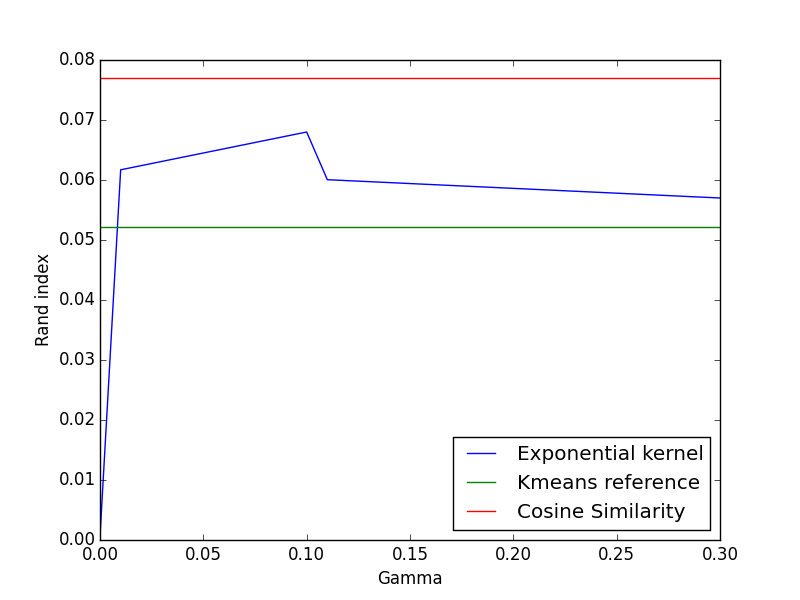
\includegraphics[width=0.8\linewidth]{../REPORT/results.png}  
\end{figure}
\end{frame}

\begin{frame}
\frametitle{Data samples distribution ground truth}
\begin{center}
\begin{tabular}{ |c|c|c|} 
\hline
Cluster Label & Name Entity & Number of sample\\
\hline
0 & Organization & 7953\\
 \hline
1 & Location & 4743\\
 \hline
2 & Person & 5314\\
 \hline
3 & Miscellaneous & 2441\\
 \hline
\end{tabular}
\end{center}
\end{frame}



\begin{frame}
\frametitle{Confusion matrix}
\begin{figure} 
  \label{confusion} 
  \begin{minipage}[b]{0.5\linewidth}
    \centering
    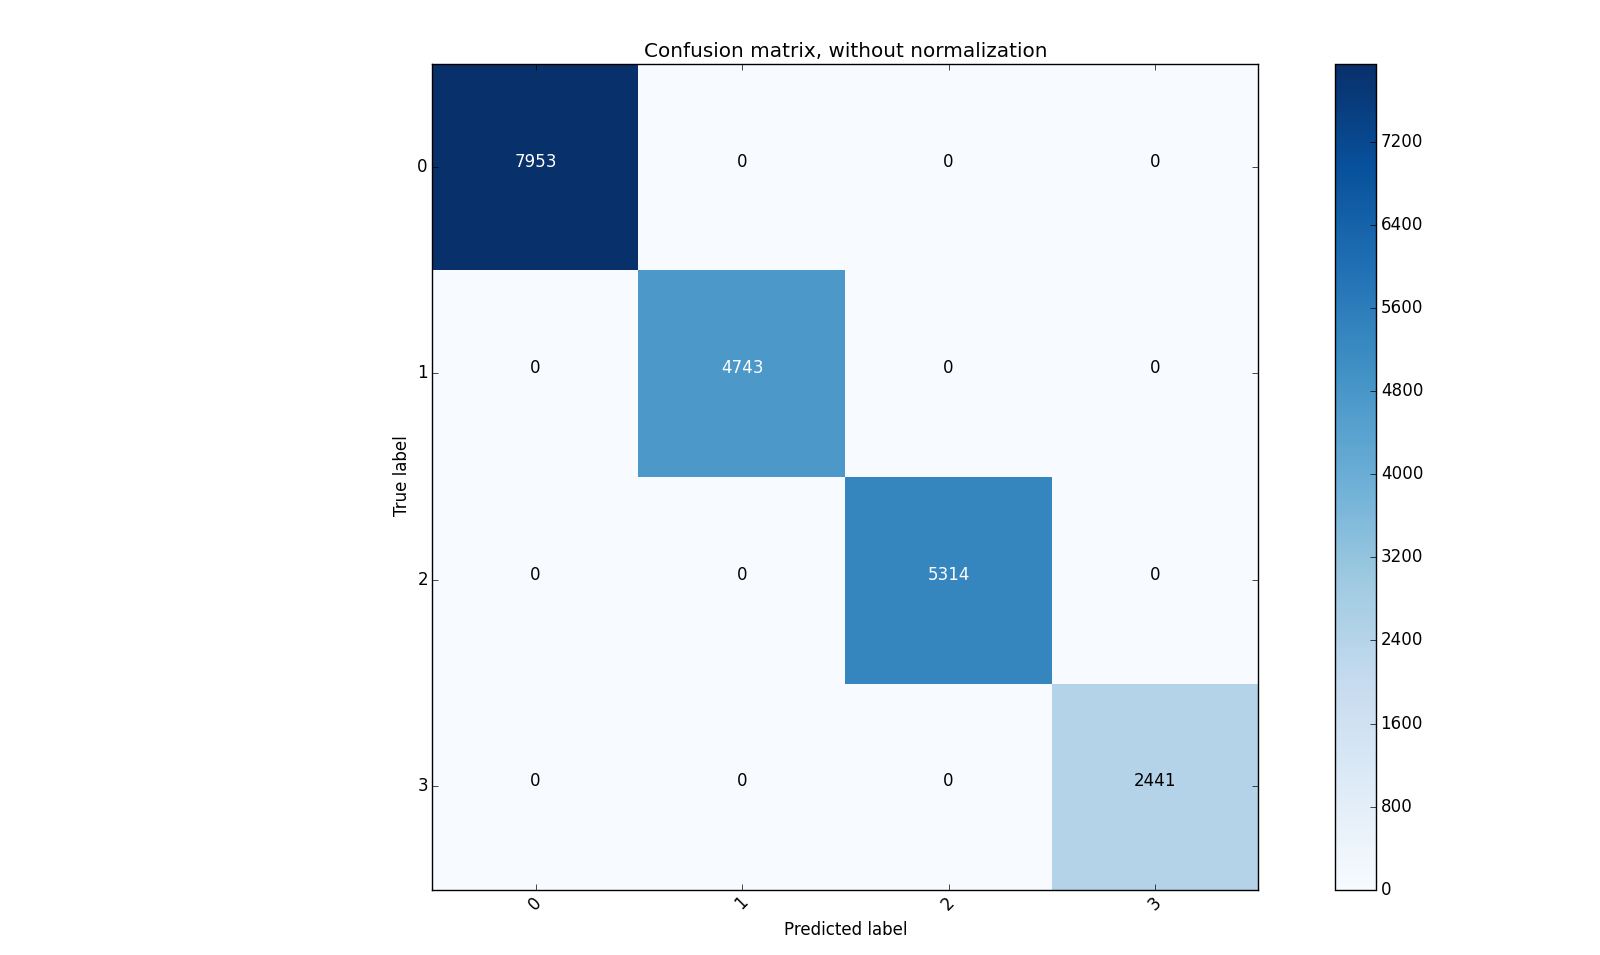
\includegraphics[width=1\linewidth]{../REPORT/label_distribution.png} 
%    \caption{True label distribution} 
    \vspace{2ex}
  \end{minipage}%%
  \begin{minipage}[b]{0.5\linewidth}
    \centering
    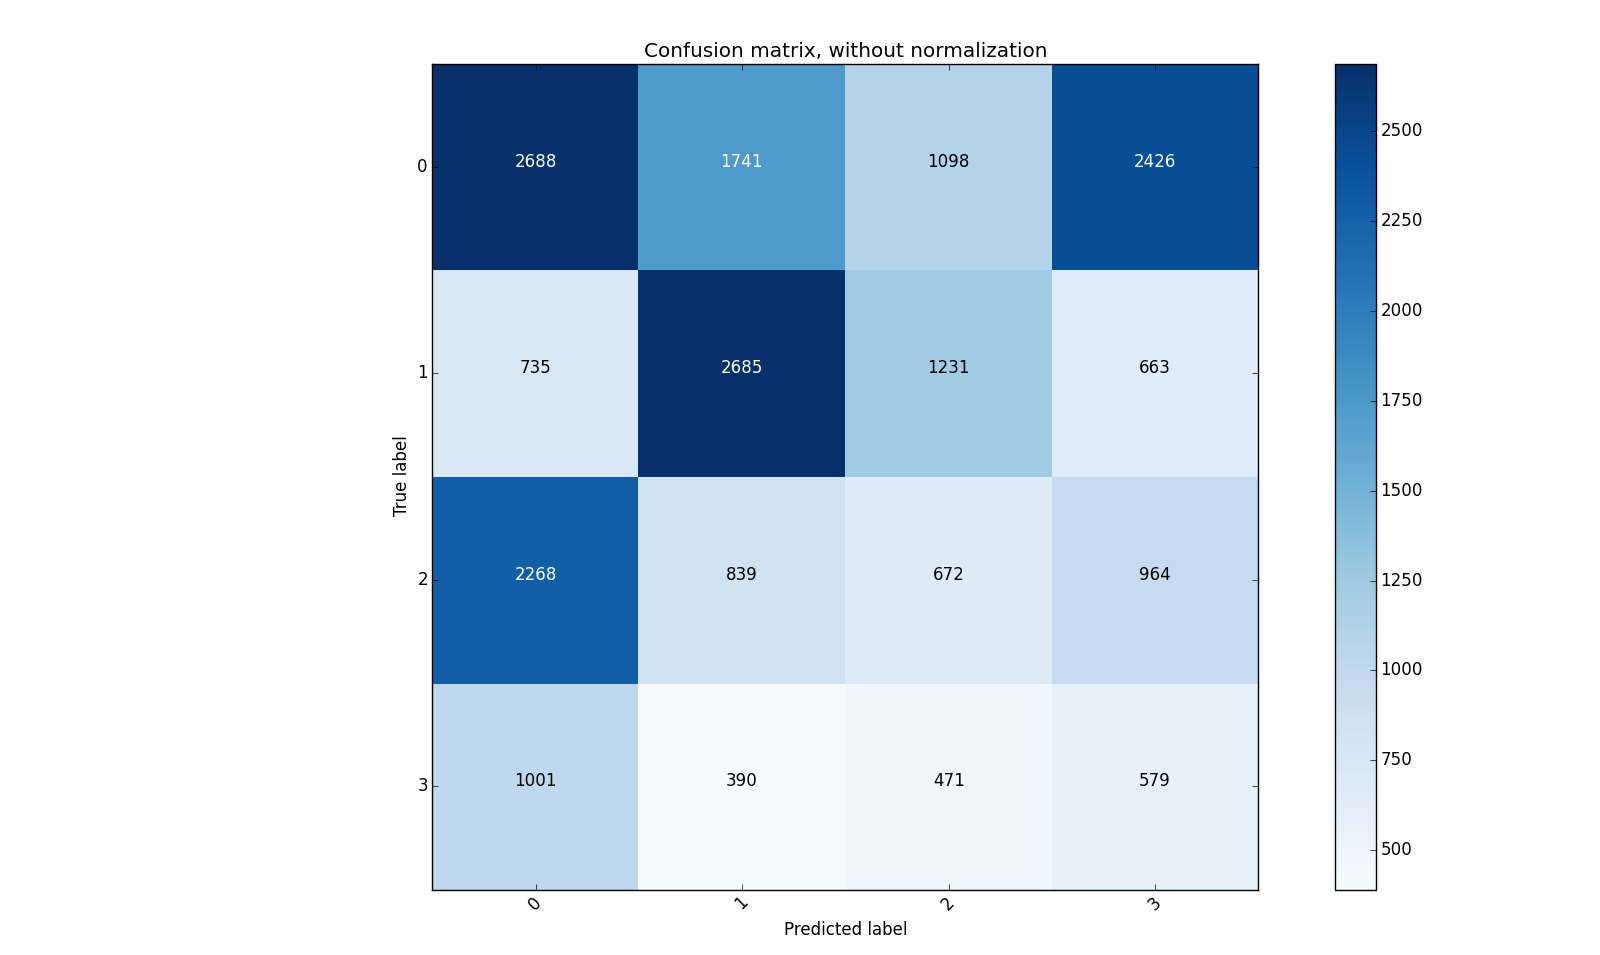
\includegraphics[width=1\linewidth]{../REPORT/kmeans2.png} 
   % \caption{Kmeans Clustering} 
    \vspace{2ex}
  \end{minipage} 
  \begin{minipage}[b]{0.5\linewidth}
    \centering
    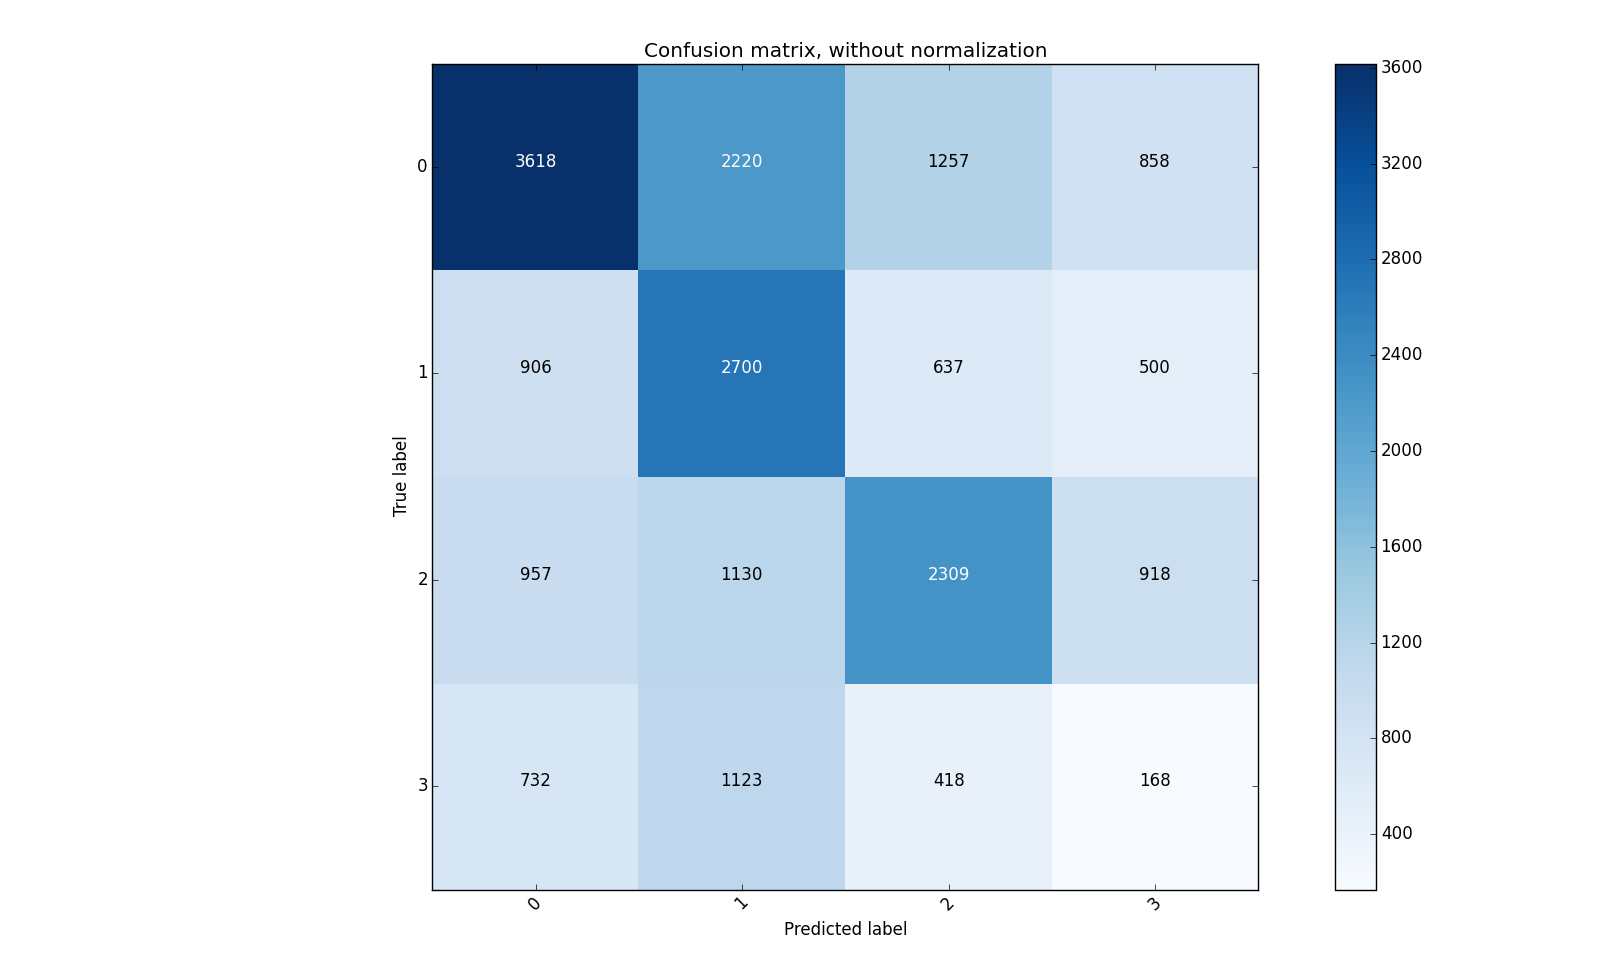
\includegraphics[width=1\linewidth]{../REPORT/bestModel2.png} 
    %\caption{Spectral(exponential kernel)} 
    \vspace{2ex}
  \end{minipage}%% 
  \begin{minipage}[b]{0.5\linewidth}
    \centering
    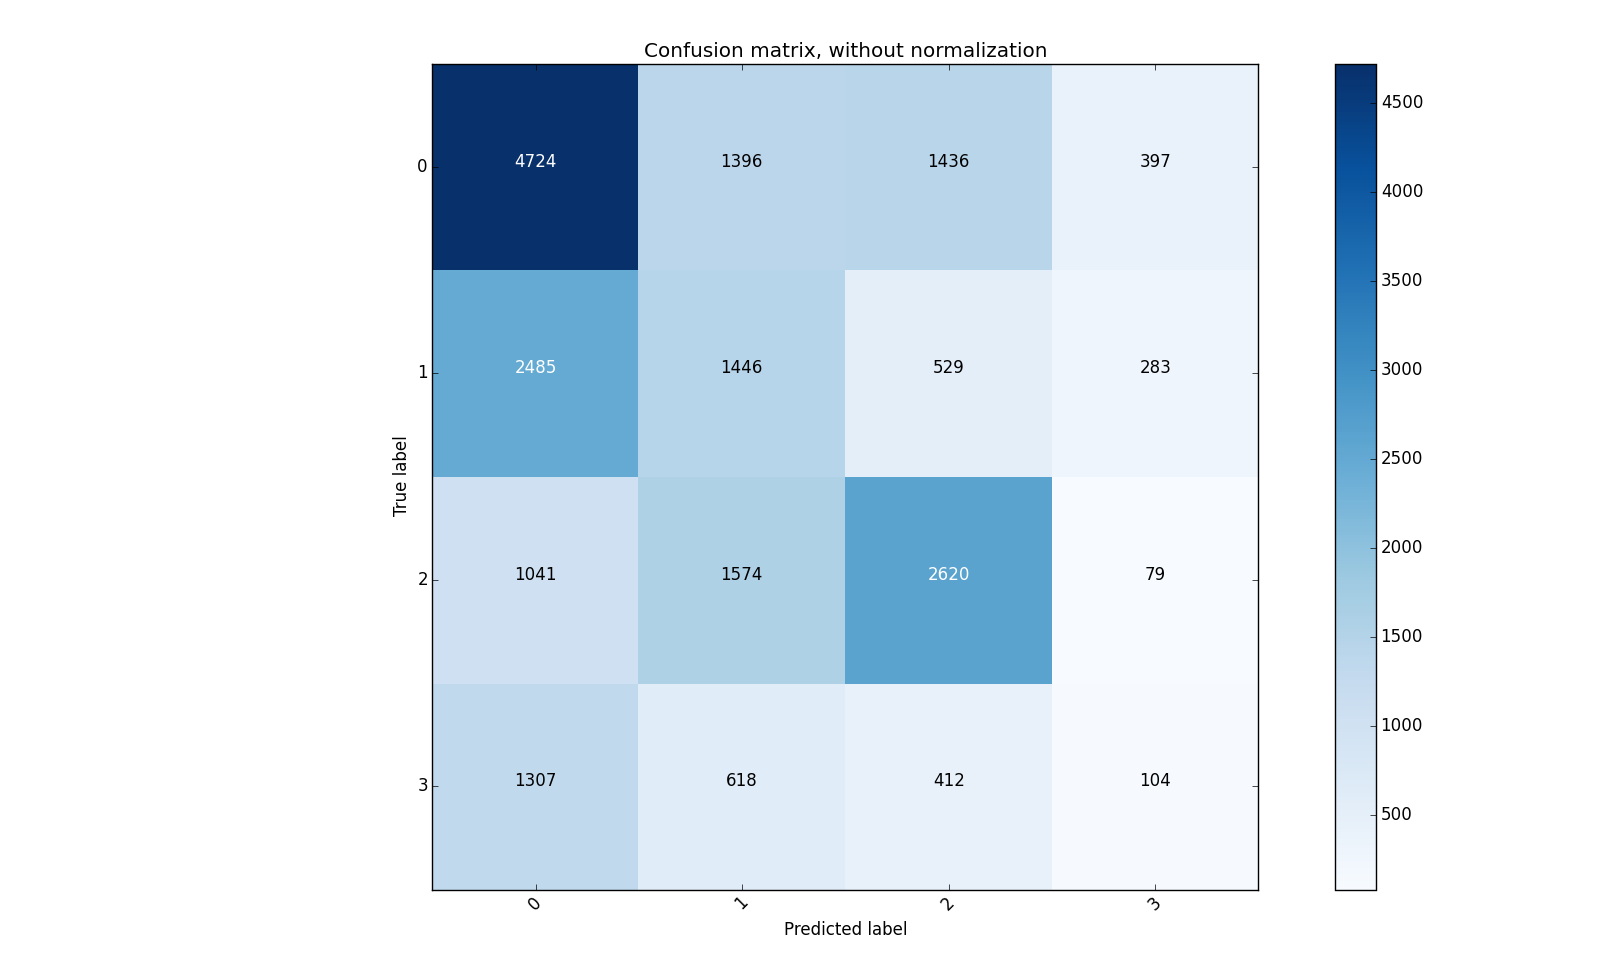
\includegraphics[width=1\linewidth]{../REPORT/cosSimConfMat2.png} 
    %\caption{Spectral(Cosine similarity)} 
    \vspace{2ex}
  \end{minipage} 
\end{figure}
\end{frame}


\begin{frame}
\frametitle{Data visualisation in 2d}
\begin{figure}
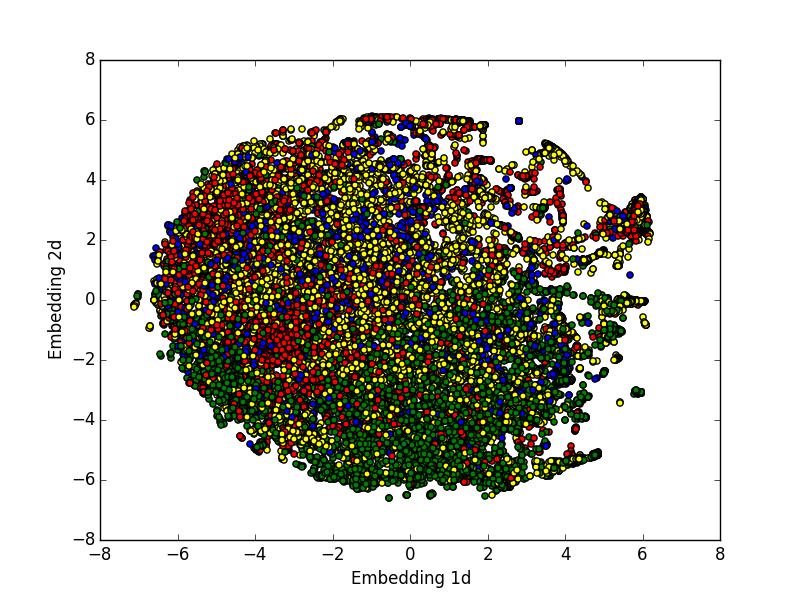
\includegraphics[width=0.8\linewidth]{../REPORT/embedding2DTrue_labelsColor2.png}  
\end{figure}
\end{frame}


\begin{frame}
\frametitle{Conclusion}
\begin{itemize} 
\item bleble
\item bleble
\end{itemize}
\end{frame}



 
 
 

\end{document} 